\section{问题二：历史预测与两日滚动购电}
\subsection{面向费用的历史组合预测}
在零点尚不知道当天实际负荷与光伏，因此根据周周期与短期持续性构造
\begin{align}
\widehat L_{d,t}&=w_{d,1}L_{d-7,t}+w_{d,2}L_{d-14,t}+w_{d,3}\bar L_t,\label{eq:load}\\
\widehat P_{d,t}&=u_{d,1}P_{d-1,t}+u_{d,2}P_{d-2,t}+u_{d,3}\bar P_t,\label{eq:pv}
\end{align}
其中$\bar L_t,\bar P_t$为题目给定典型日电量，权重非负且各自和为1。
两组三源权重在步长0.2的单纯形网格搜索，共$21\times21=441$个组合。
令$C_j(w,u)$为历史日$j$使用该权重作计划并以实际值因果执行后的总费用，递推评分为
\begin{equation}
\begin{aligned}
M_d(w,u)&=\rho M_{d-1}(w,u)+(1-\rho)C_{d-1}(w,u),\\
\rho&=2^{-1/h},\qquad (w_d,u_d)=\arg\min_{w,u}M_d(w,u).
\end{aligned}
\label{eq:ewma}
\end{equation}
历史首个可用评分初始化$M$，随后每日只吸收前一日实现费用。半衰期取$h=5$天。
历史成本表采用单日规划、自由末端执行的代理费用，正式运行采用两日滚动，二者不能视为完全相同的优化目标；这种代理降低了逐日权重标定的计算量。

为控制高价短缺，对预测施加
\begin{equation}
\widetilde L_{d,t}=\kappa\widehat L_{d,t},\qquad
\widetilde P_{d,t}=[\widehat P_{d,t}-m\Delta t]_+,
\quad \kappa=1.02,\ m=25\ {\rm kW}.
\label{eq:margin}
\end{equation}
若忽略储能与跨期耦合，仅考虑计划量$z$和随机净需求$N$，最小化
$pz+5p\,\mathbb E[(N-z)_+]$给出$F_N(z)=0.8$。
这解释了保守修正的方向，但不能据此直接确定含储能模型的最优裕度；具体参数仍由历史开发期费用选择。
\subsection{两日计划及次日预测}
每日以实际日初电量$E_{d,0}$初始化288槽规划，目标为
\begin{equation}
\min\sum_{\tau=1}^{288}\widehat p_\tau x_\tau+
\varepsilon\sum_{\tau=1}^{288}(c_\tau+q_\tau),
\label{eq:rolling}
\end{equation}
并对预测负荷、光伏施加式\eqref{eq:balance}--\eqref{eq:bounds}。
微小吞吐量正则项用于减少无意义充放循环，报送购电费不含此数值求解罚项。
当日末$E_{144}$和窗口最远端$E_{288}$均不设置等式终值，仅满足容量界限。
次日负荷利用$d+1-7,d+1-14$的已发生曲线，当日冻结的光伏权重应用于截至$d-1$的最近两条实际曲线；禁止使用当天尚未发生的光伏来构造次日预测。
\subsection{逐槽因果执行}
固定当前有效承诺量$x_t$，观察当前实际负荷和光伏，记
$n_t=L_t-P_t-x_t$。当$n_t\geq0$时，
\begin{equation}
q_t=\min\{n_t,\bar c,\eta(E_{t-1}-1200)\},\quad
e_t=n_t-q_t,\quad c_t=s_t=0.
\label{eq:discharge}
\end{equation}
当$n_t<0$时，
\begin{equation}
c_t=\min\{-n_t,\bar c,(10800-E_{t-1})/\eta\},\quad
s_t=-n_t-c_t,\quad q_t=e_t=0.
\label{eq:charge}
\end{equation}
然后按式\eqref{eq:soc}更新储电量。这一规则只依赖当前槽及此前信息，不为追赶日末目标而额外紧急购电充能。
次日初值为本日实际末值：
\begin{equation}E_{d+1,0}=E_{d,T}^{\rm exec}.\label{eq:crossday}\end{equation}
计划富余不会退费，故实现费用为
\begin{equation}C_2=\sum_d\sum_t p_t x^0_{d,t}+5\sum_d\sum_t p_t e_{d,t}.\label{eq:q2cost}\end{equation}
\subsection{时间留出选择与总费用}
2月至6月为开发期，7月至12月为验证期；后者只报告性能，不用于重新选择全局参数。
表\ref{tab:holdout}显示相邻候选表现接近。所选$m=25$在开发期最优，在验证期排名第5；$m=50$的全年描述值略低，也不能据此倒过来改选。
因此334天汇总包括开发期，不能称为全区间独立样本外测试。
\begin{table}[htbp]\centering
\caption{问题二部分候选的时间留出结果（万元，均为$h=5$）}\label{tab:holdout}
\begin{tabular}{ccrrrr}
\toprule
$\kappa$ & $m$/kW & 开发期 & 验证期 & 全区间 & 验证排名\\\midrule
1.02 & 25（选定） & 574.0 & 821.6 & 1395.7 & 5\\
1.02 & 50 & 574.2 & 820.6 & 1394.8 & 4\\
1.015 & 75 & 574.3 & 821.7 & 1396.1 & 6\\
1.02 & 75 & 575.0 & 820.3 & 1395.3 & 2\\
\bottomrule
\end{tabular}
\end{table}
正式结果总费用1395.7万元，其中计划购电费1316.0万元、紧急购电费79.6万元；分项独立舍入可能与总额相差0.1万元。
图\ref{fig:q2soc}给出储能轨迹，日末值随供需变化而变化，验证了跨日状态连续与非固定末端条件。
\begin{figure}[htbp]\centering
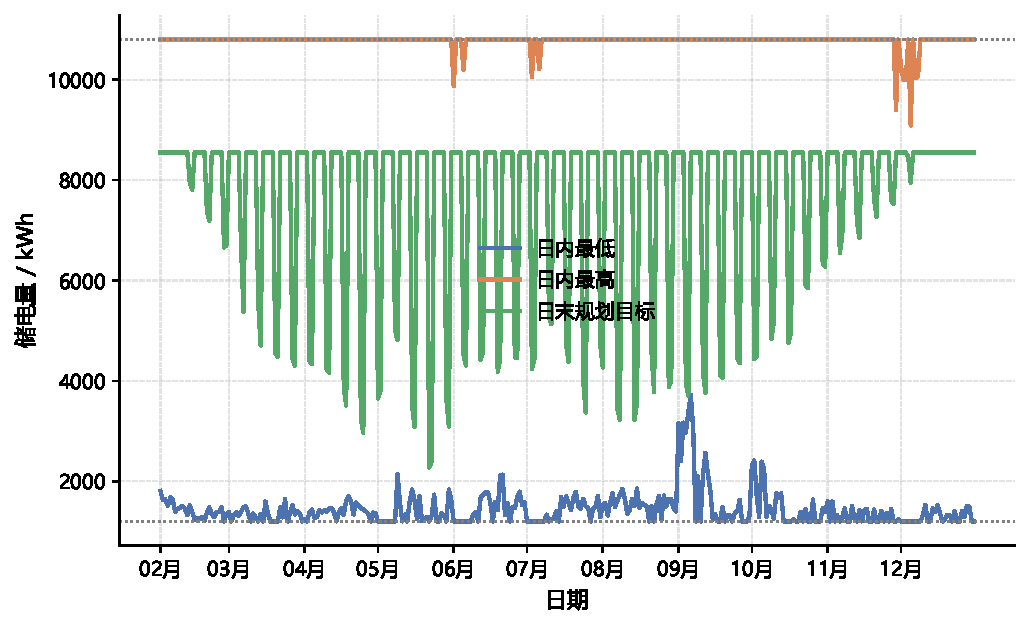
\includegraphics[width=.91\textwidth]{../../figures/Q2_储能轨迹.pdf}
\caption{问题二实际储能电量及日末电量变化}\label{fig:q2soc}
\end{figure}
\subsection{指定日期结果与年度风险}
四个指定日期的计划购电、储能与紧急购电结果见表\ref{tab:q2buy}--\ref{tab:q2emerg}。
计划购电费与包含紧急费的总费用分别列示，以保持题目结算含义。
\begin{table}[htbp]\centering
\caption{问题二指定日期计划购电量与购电费}\label{tab:q2buy}
\small
\begin{tabular}{lrrrr}
\toprule
时段或指标 & 3月20日 & 6月21日 & 9月23日 & 12月21日 \\
\midrule
10:00-10:10 & 0.00 & 0.00 & 0.00 & 0.00 \\
12:00-12:10 & 529.03 & 0.00 & 553.22 & 975.48 \\
14:00-14:10 & 0.00 & 0.00 & 0.00 & 0.00 \\
16:00-16:10 & 428.10 & 169.90 & 464.46 & 796.72 \\
18:00-18:10 & 744.10 & 534.28 & 802.45 & 731.57 \\
20:00-20:10 & 0.00 & 0.00 & 0.00 & 0.00 \\
全天计划电量/kWh & 62281.59 & 42865.34 & 69038.87 & 96267.73 \\
全天计划购电费/元 & 38733.07 & 24447.24 & 42750.14 & 61810.51 \\
紧急购电费/元 & 1592.53 & 0.00 & 1003.07 & 83.06 \\
含紧急费总额/元 & 40325.60 & 24447.24 & 43753.21 & 61893.57 \\
\bottomrule
\end{tabular}
\end{table}
\begin{table}[htbp]\centering
\caption{问题二指定日期储能充放电与首末电量（kWh）}\label{tab:q2soc}
\footnotesize
\setlength{\tabcolsep}{4pt}
\begin{tabular}{lrrrrrrrr}
\toprule
 & \multicolumn{2}{c}{3月20日} & \multicolumn{2}{c}{6月21日} & \multicolumn{2}{c}{9月23日} & \multicolumn{2}{c}{12月21日}\\
区间 & 充电 & 放电 & 充电 & 放电 & 充电 & 放电 & 充电 & 放电 \\
\midrule
0:00-4:00 & 1376.88 & 122.05 & 447.73 & 200.31 & 2042.44 & 43.58 & 2040.21 & 276.70 \\
4:00-8:00 & 992.89 & 4988.27 & 593.50 & 1782.09 & 405.75 & 6608.26 & 1608.84 & 1579.87 \\
8:00-12:00 & 5356.38 & 2777.38 & 7656.06 & 0.00 & 5589.93 & 1896.62 & 5310.48 & 7513.53 \\
12:00-16:00 & 4272.48 & 534.09 & 0.00 & 0.00 & 5123.65 & 597.06 & 7804.74 & 2276.46 \\
16:00-20:00 & 313.91 & 5924.64 & 242.20 & 5524.96 & 213.59 & 5649.98 & 0.00 & 5685.08 \\
20:00-24:00 & 4089.80 & 2792.53 & 8635.18 & 2570.34 & 8474.10 & 2826.51 & 8405.16 & 2848.38 \\
0:00电量 & \multicolumn{2}{c}{9061.33} & \multicolumn{2}{c}{5175.11} & \multicolumn{2}{c}{8709.06} & \multicolumn{2}{c}{8652.78} \\
24:00电量 & \multicolumn{2}{c}{4780.15} & \multicolumn{2}{c}{9794.87} & \multicolumn{2}{c}{8793.57} & \multicolumn{2}{c}{8883.03} \\
\bottomrule
\end{tabular}
\end{table}
\begin{table}[htbp]\centering
\caption{问题二指定日期全部紧急购电事件}\label{tab:q2emerg}
\small
\begin{tabular}{ccr}
\toprule
日期 & 紧急购电时段 & 紧急购电量/kWh \\
\midrule
03月20日 & 20:30-20:40 & 228.2867 \\
06月21日 & 无 & 0.0000 \\
09月23日 & 20:20-20:40 & 103.1061 \\
09月23日 & 20:50-21:10 & 43.2148 \\
09月23日 & 21:20-21:40 & 17.9760 \\
12月21日 & 7:50-8:00 & 14.2992 \\
\bottomrule
\end{tabular}
\end{table}

固定已生成的两日滚动计划，对负荷和光伏联合残差作同月整日块重采样，得到100个模拟评价年度。
这种模拟是条件于固定计划的离线压力评估，不是重新训练并逐年适应的独立样本外试验。
总成本均值1464万元，标准差44.53万元，P95为1542万元，尾部均值CVaR95为1566万元。
CVaR刻画超过分位阈值的平均损失\cite{rockafellar2000}，适合补充均值指标。
\begin{figure}[htbp]\centering
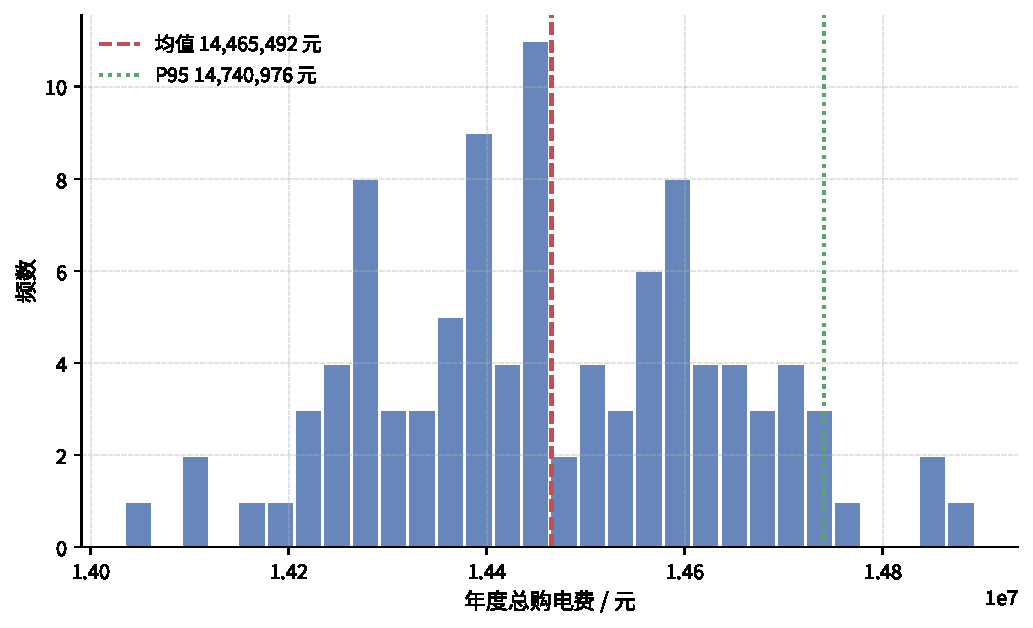
\includegraphics[width=.75\textwidth]{../../figures/Q2_总费用分布.pdf}
\caption{固定计划下联合残差重采样的总费用分布}\label{fig:q2risk}
\end{figure}
图\ref{fig:q2risk}表明实际评价区间的1395.7万元低于重采样均值，不能把这一实现值直接等同于未来期望成本。
\questionconclusion{基于开发期选择的历史预测与两日滚动策略在334天内产生1395.7万元费用；实际末端电量自由，风险评价仍显示明显的高费用尾部。}
